% Sample pages for Ceyhun Cizge Kurami

% Haluk Bingol
% v20161028

\documentclass[11pt]{amsbook}
\usepackage[turkish]{babel}

\usepackage{../Ceyhun}	% ------------------------
\usepackage{../amsTurkish}


\usepackage{lipsum}



\begin{document}
% ++++++++++++++++++++++++++++++++++++++
\hPage{016}
% ++++++++++++++++++++++++++++++++++++++
% =======================================
kapalı olmayan dolaşılara \underline{\itshape{açık dolaşı}} $\hAbs{D_{i,j}}$ ile göstereceğimiz dolaşıdaki ayrıtların sayısına dolaşının \underline{\itshape{uzunluğu}} diyeceğiz.  \\
\reffig{1.2.1} deki $Ç(9.14)$ çizgesinde
$$D_{1,5} = \hPairingParan{a_1,a_7,a_{11},a_{14},a_1,a_7,a_6,a_5,a_2,a_7,a_8,a_9,a_4,a_4}$$
uç düğümleri $d_1$ ve $d_5$, uzunluğu ise 14 olan ve $a_1,a_2,a_4,a_5,a_6,a_7,a_8,a_9,a_{11},a_{14}$ ayrıtlarından oluşan bir dolaşıdır. Bu dolaşıda; $a_2,a_5,a_6,a_8,a_9,a_{11},a_{14}$ tekkatlı; $a_1,a_4$ 2-katlı ve $a_7$ 3-katlı ayrıtlardır.

\begin{definition}
Yalnız tekkatlı ayrıtlardan oluşan dolaşıya \underline{\itshape{gezi}} $\hPairingParan{G_{i,j}}$ denir.
\end{definition}

Dolaşıda olduğu gibi $G_{i,j}$ geszisi için de; \itshape{uç düğümler, açık gezi, kapalı gezi, ve gezi uzunluğu} $\hPairingParan{\hAbs{G_{i,j}}}$ kavramları benzer olarak tanımlanır.

 \begin{figure}[hb]
 	\centering
 	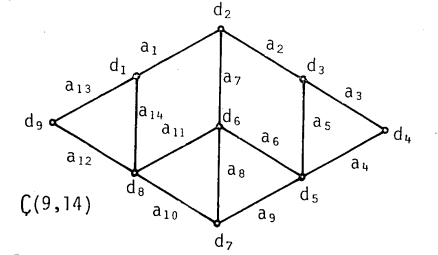
\includegraphics[width=0.45\textwidth]{images/ceyhun-016}
 	\caption{Dolaşının açıklanması.}
 	\label{1.2.1}
 \end{figure}
% =======================================================
\end{document}  